\documentclass[resume]{subfiles}


\begin{document}
\begin{multicols}{3}
\section{PCB}
\subsection{Général}
\paragraph{Circuit haute vitesse} : $t_r < 2\tau$ avec $t_r$ le temps de montée / descente et $\tau$ le temps de propagation ($L > \lambda/2$)\\
$\rightarrow$ prendre en compte les effets de la ligne de transmission
$$\tau=\frac{L}{\nu_{ph}}$$
Avec $\nu_{ph}$ la vitesse de propagation (typiquement $0.5$...$0.6c$)
$$\nu_{ph}=\frac{c}{\sqrt{\epsilon_r\mu_r}}$$
$$c\approx 3\cdot 10^{8}$$
\paragraph{Extérieur} : Câbles, connecteurs, composants plus grands que $\lambda/10$
\paragraph{Sources de bruit} : PWM, bruit GND, oscillateurs, RF, spurious signals
\paragraph{Mesures de protection} : ferrites, filtres, opto-coupleurs, chokes, fibres optiques, R / L en série, shields, condensateurs, ferites au dela de \SI{100}{\mega\hertz}, stitching
\subsection{Guides d'ondes}
$$a=\frac{\lambda_c}{2}\qquad \lambda_c=\frac{c}{f_c}$$
$f_c$ la fréquence de transmission. Atténuation faible au delà et faible avant. Stitching $<\lambda/2$ pour éviter l'entrée / sortie d'ondes dans le pcb.\\
Transformation d'un guide d'onde en câble coax lorsqu'on place un conducteur interne
\subsection{Blindage}
Matériau du blindage, résonances, nombres de points de contact avec le plan GND.\\
Comment protéger la partie intérieur d'un pcb? en divisant les zones, en blindant les composants sensibles et en filtrant les signaux des parties internes
\subsection{Connecteurs}
\begin{figure}[H]
\centering
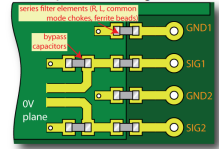
\includegraphics[width=4.00cm]{img_0.png}
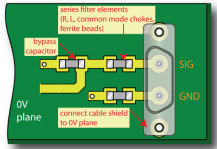
\includegraphics[width=4.00cm]{img_1.png}
\caption{Câble non-blindé vs câble blindé}
\end{figure}
\subsection{Filtrage}
\begin{figure}[H]
\centering
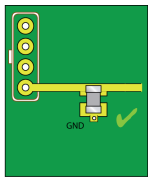
\includegraphics[width=2.00cm]{img_2.png}
\end{figure}
\subsection{Courant}
Chemin de retour du courant sur le plan le plus proche du signal (distribution gaussienne centrée sur la piste du signal). Si plusieurs chemins ou trop d'écartement $\longrightarrow$ tension/courant en mode commun et/ou bruit GND.\\
Il faut que le chemin de retour soit aussi proche que possible du chemin d'aller.
Les signaux différentiels produisent moins de perturbations et sont moins perturbés
\paragraph{Bruit en mode commun} (common mode current) peut être généré par une série d'impédance dans la ligne de retour, par des charges parasites, par du bruit externe au circuit, etc. Le mode commun peut se traduire comme le mode différentiel et peut produire des chutes de tensions non désirées sur une charge. Réduire l'impédance du GND, éviter les faux chemins de retour
\paragraph{Causes de courant en mode commun}
\begin{enumerate}
\item Retour par un plan de masse de section faible
\item Capacités différentes sur paires différentielles
\item Sources externes
\item Impédances différentes sur l'aller et le retour
\end{enumerate}
\paragraph{Plan image} terme pour une couche pleine (masse ou alim). Sert de chemin de retour pour les pistes des autres couches. 
\subsection{Pistes}
$R=\SI{19}{\milli\ohm\per\centi\meter}$ pour \SI{0.254}{\milli\meter} de largeur et \SI{35}{\micro\meter} d'épaisseur
\subsubsection{Stripline}
\begin{figure}[H]
\centering
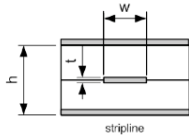
\includegraphics[width=3.00cm]{img_15.png}
\end{figure}
$$Z_0\approx\frac{60}{\sqrt{\varepsilon_r}}\ln\left(\frac{4h}{0.67\pi w\left(0.8+t/w\right)}\right)$$
$$\nu_{ph}\approx\frac{0.3048}{1.017\sqrt{\varepsilon_r}}\ [\si{\meter\per\nano\second}]$$
\subsubsection{Microstrip}
\begin{figure}[H]
\centering
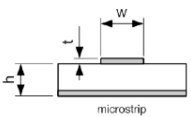
\includegraphics[width=3.00cm]{img_16.png}
\end{figure}
$$Z_0\approx \frac{87}{\sqrt{\varepsilon_r+1.41}}\ln\left(\frac{5.98h}{0.8w+t}\right)$$
$$\nu_{ph}\approx\frac{0.3048}{1.017\sqrt{0.457\varepsilon_r+0.67}}\ [\si{\meter\per\nano\second}]$$

\paragraph{Méthodologie} : Définition des couches, Placer les connecteurs et les vis, Placer les composants critiques, Zones du PCB (numérique, analogique), Layout.\\
\paragraph{Résistance}
$$R = \rho \frac{Z(\text{\scriptsize longueur})}{X(\text{\scriptsize largeur})Y(\text{\scriptsize hauteur})}\qquad \rho\approx\SI{0.0175}{\ohm\square\milli\meter\per\meter}$$
\begin{figure}[H]
\centering
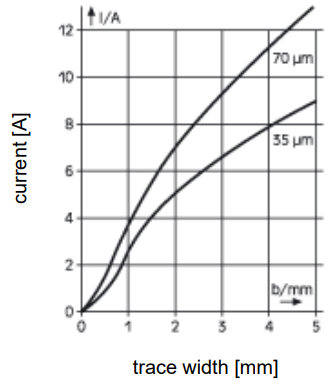
\includegraphics[width=4.00cm]{img_10.png}
\end{figure}
\paragraph{Inductance}
\begin{figure}[H]
\centering
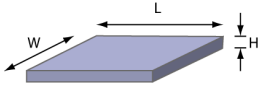
\includegraphics[width=4.00cm]{img_11.png}
\end{figure}
\begin{scriptsize}
$$L_0=\frac{2}{10^{4}}L\left(\ln\left(\frac{2L}{W+H}\right)+0.2235\left(\frac{W+H}{L}\right)+0.5\right)\ [\si{\micro\henry}]$$
\end{scriptsize}
\paragraph{Inductance mutuelle (M)}
\begin{align*}
V_1&=L\frac{di_1}{dt}+M\frac{di_2}{dt}\\
V_2&=L\frac{di_2}{dt}+M\frac{di_1}{dt}
\end{align*}
\begin{figure}[H]
\centering
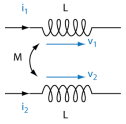
\includegraphics[width=4.00cm]{img_12.png}
\end{figure}
\subsection{Couches}
\begin{enumerate}
\item S-G-V-S (économie de vias, bonne protection)
\item S-G-S-B (pas symétrique, très bonne protection)
\item G-S-S-V (beaucoup de vias, trous dans les plans)
\end{enumerate}
Si $f>\SI{5}{\mega\hertz}$ ou $t<\SI{5}{\nano\second}$ alors il faut utiliser un pcb multicouches.\\
Rapprocher les couches GND et VCC pour maximiser le découplage. Les plans images (GND, VCC) doivent être proches de couches de signaux.
\subsubsection{Empilements à utiliser}
Toujours avoir un système symétrique (pour éviter que le board se torde après usinage).\\
réduction de la distance entre couche signaux et couche plan permet de rendre les signaux plus robustes face aux perturbations
\begin{enumerate}
\item S-G-V-S
\item S-G-S--S-V-S
\item S-G-V-S-S-V-G-S
\end{enumerate}
\subsection{Antennes}
Champ électrique $E$ généré par une boucle d'aire $A$ traversée par un courant $I$ à une distance $R$
$$E\sim \frac{k^2 IA}{4\pi}\sqrt{\frac{\mu}{\epsilon}}\left(\frac{1}{R}\right)\qquad k=\frac{2\pi}{\lambda}=\frac{\omega}{c}$$
\subsubsection{Antenne dipôle}
\begin{figure}[H]
\centering
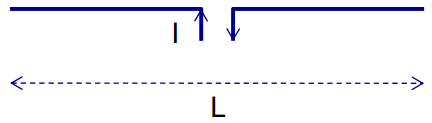
\includegraphics[width=3.00cm]{img_5.png}
\end{figure}
$$E\sim \frac{ILf}{4\epsilon_0 R}$$
\subsubsection{Antenne "slot"}
\begin{figure}[H]
\centering
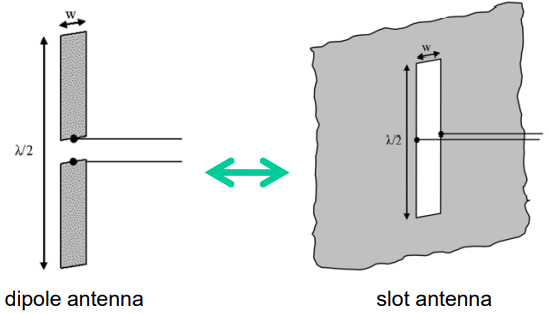
\includegraphics[width=6.00cm]{img_6.png}
\end{figure}
$$f=\frac{c}{\lambda\sqrt{\varepsilon_r}}$$
FR-4 : $\varepsilon_r=4\quad (2.5...6)$
\subsection{Horloge}
\begin{itemize}
\item Mêmes longueurs de pistes (distribution en étoile)
\item Ne pas traverser des trous dans le GND
\item Blindage éventuel pour éviter le rayonnement (signaux analogiques faibles).
\end{itemize}
\subsubsection{Jitter}
Petites variation d'un oscillator. Le jitter contribue à réduire le rapport signal sur bruit
$$\text{SNR}=20\log_{10}\left(\frac{1}{2\pi ft_\text{jitter}}\right)$$
\subsubsection{Skew}
Différence de temps pour que le signal atteigne les différents ICs.\\
Pour éviter ça, mettre le distributeur de clock au centre et distribuer avec des longueurs de piste égales.
\subsubsection{Distribution}
\begin{figure}[H]
\centering
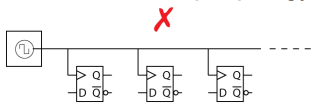
\includegraphics[width=4.00cm]{img_26.png}
\end{figure}
\begin{figure}[H]
\centering
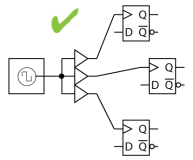
\includegraphics[width=4.00cm]{img_27.png}
\end{figure}

\subsubsection{Émissions}
L'horloge peut émettre des perturbations si :
\begin{itemize}
\item Il existe des boucles de retour de courant
\item L'horloge traverse des antennes slot
\end{itemize}
Si on doit traverser une fente, on peut ajouter un condensateur.


\subsection{Découplage}
Atténuation des perturbations d'IC et/ou charge de capacités pour diminuer les perturbations et/ou garantir le fonctionnement du système. Placer des capa entre GND et VCC.\\
Le circuit équivalent d'une capacité est un circuit ESR(R)-ESL(L)-C en série. ESL + C forment une circuit résonant en série. Au dessus de $\omega_{resonance}$, la capa agit comme une inductance. ESL dépend du format et de la taille de la capa.\\
$$\omega_{res}=\frac{1}{\sqrt{LC}}$$
\begin{figure}[H]
\centering
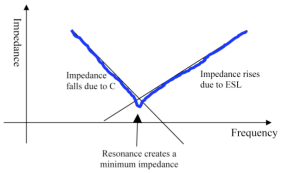
\includegraphics[width=4.00cm]{img_7.png}
\end{figure}
Comment choisir la capacité de découplage? utiliser des multicouche céramique, le plus petit format possible, généralement : 100nF, 10nF, 1 nF\\
\begin{figure}[H]
\centering
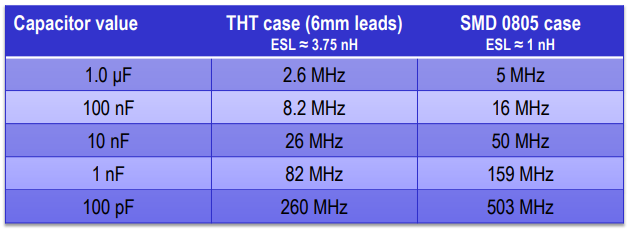
\includegraphics[width=5.00cm]{img_8.png}
\end{figure}
On souhaite un grand ESR pour avoir une atténuation lors de la mise en parallèle (résonance parallèle) et un ESL petit pour avoir la plus fréquence de coupure le plus haut possible.\\
Lors de la mise en parallèle des capa, disposer les capa en tête-bêche (flux de courant en sens opposés) pour annuler les champs magnétiques émis mutuellement.\\
Si les plans d'alimentation pour la partie analogique et la partie numérique sont séparés, les relier avec des ferrites.\\
Gros condensateur (\SIrange{10}{50}{\micro\farad}) pour découpler l'alimentation et petit (\SI{100}{\nano\farad}) pour les hautes fréquences
\subsubsection{Placement du condensateur}
\begin{figure}[H]
\centering
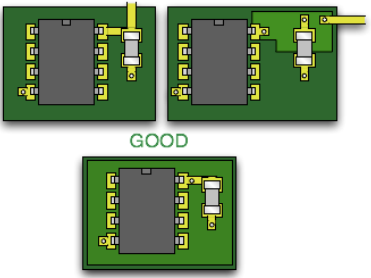
\includegraphics[width=5.00cm]{img_9.png}
\end{figure}
Garder les connexions courtes, éviter de mettre les condensateurs dans le même sens, placer les vias directement dans les pads si nécessaire.
\subsection{Plans}
Capacité intrinsèque entre les plans :
$$C=\varepsilon_0\varepsilon_r\frac{A}{d}$$
Éviter la résonance des plans en choisissant un rapport longueur / largeur irrationnel.
\subsection{Plan de masse}
\paragraph{Masse chaude} : fait le tour du circuit (vis, connecteurs)
\paragraph{Masse froide} : GND interne du circuit
Les deux masses sont reliées par un pont qui empêche le passage des perturbations.\\
Il faut éviter les interruptions du plan de masse (surtout si elles sont longues).\\
Lorsqu'il y a plusieurs plans de masse (AGND, DGND), on utilise une connexion en étoile. Si l'impédance du plan de masse est assez faible on peut les fusionner\\
Remplir toutes les zones non-utilisées par des plans de masse (ou de VCC).\\
Attention aux pass-through vias sont des "bouchons" et des antennes emettrices. Elles créent des trous dans le plan de référence et réduisent l'effet de blindage
\subsubsection{Séparation des plan de masse}
\begin{multicols}{2}
\begin{enumerate}[label={+}]
\item isolation de zones (analogique sensible, connections à des appareils bruyants)
\item Contrôle des chemin de retour 
\item Réduction des capacités parasites
\end{enumerate}
\begin{enumerate}[label={-}]
\item Les coupures peuvent générer des antennes
\item Pas forcément utile
\end{enumerate}
\end{multicols}
Stitching avec une distance $\lambda/10$ pour améliorer la protection des zones sensibles.\\
Pour connecteur deux plans, utiliser des capa si le signal est rapide et des inductances si le signal est lent.\\
Relier deux plans de masse séparés par deux diodes Schottky tête-bêche ou par des ferrites
\subsection{Lignes de transmission}
Impédance caractéristique à HF (impédance de la ligne non fermée, si elle possédait une longueur infinie) :
$$Z_0\approx \sqrt{\frac{L'}{C'}} $$
Vitesse de propagation :
$$\nu_{ph} = \frac{c}{\sqrt{\epsilon_r \mu_r}} = \frac{1}{\sqrt{L' C''}}$$ avec $\mu_r = 1$ et $\epsilon_r =4...4.5$\\
Avant réflexion, on a $u_a$ et $i_a$. Pour éviter les réflexions ont doit placer une charge $Z=Z_0$.\\
Prendre en compte les effets de la ligne de transmission si l'aller-retour du signal est plus grand que le temps de montée / descente du signal.\\
Éviter de changer de couche avec des signaux haute-vitesse. Si un via est inévitable, prévoir un chemin de retour non-interrompu
\subsubsection{Coefficient de réflexion}
\begin{figure}[H]
\centering
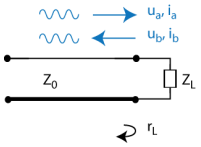
\includegraphics[width=4.00cm]{img_13.png}
\end{figure}
$$r=\frac{u_b}{u_a}$$
$$\underline{r}_L=\frac{Z_L-Z_0}{Z_L+Z_0}$$
$$\underline{Z}_L=Z_0\frac{1+\underline{r}_L}{1-\underline{R}_L}$$
$Z_L>Z_0$ réflexion positive (signal de même polarité que le signal incident est retourné), $Z_L<Z_0$ réflexion négative (signal de polarité opposée et retourné vers l'émetteur) et $Z_L=Z_0$ pas de réflexion\\
\subsubsection{Deux lignes de transmission}
$$\underline{r}_{\text{jonction}}=\frac{Z_1-Z_0}{Z_1+Z_0}$$
\begin{figure}[H]
\centering
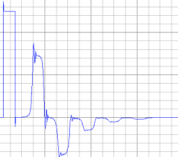
\includegraphics[width=4.00cm]{img_14.png}
\end{figure}
Un stub (bas d'un "T" fermé) : $r=1$. Un embranchement d'une ligne à deux lignes est similaire à deux résistances en parallèle. Les coins génèrent des réflexions
\subsubsection{Effet de peau}
distribution du courant (AC) que sur la surface du conducteur. Profondeur : 
$$\delta = \sqrt{\frac{2}{\omega \mu_0 \mu_r \sigma}} \qquad \sigma = 5.82\cdot 10^{7}(\text{cuivre})$$
$$R\sim \sqrt{\omega}$$
\begin{figure}[H]
\centering
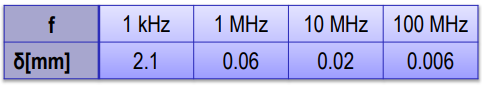
\includegraphics[width=4.00cm]{img_17.png} 
\end{figure}
\subsection{Guard ring}
entourer un nœud sensible avec un conducteur qui peut protéger des courant parasites et maintenir les conducteurs à la tension du noeud sensible. \\
\begin{figure}[H]
\centering
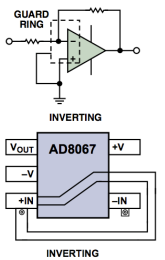
\includegraphics[width=3.00cm]{img_18.png}
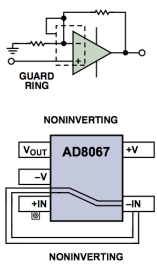
\includegraphics[width=3.00cm]{img_19.png}
\end{figure}
Il faut répéter les anneaux de garde sur chaque couche si THT
\subsection{Crosstalk}
Interférences entre des pistes proches (couplage capacitif, inductif $u=M\frac{di}{dt}$ ou retour de courant partagé avec impédance non-nulle)
\begin{figure}[H]
\centering
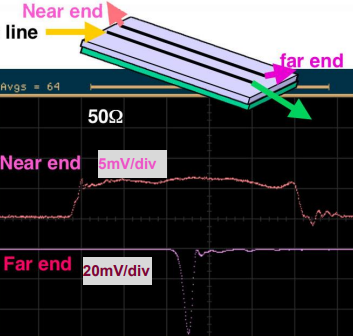
\includegraphics[width=0.9\columnwidth]{img_20.png}
\end{figure}
Pour diminuer le cross-talk on peut : éviter les pistes parallèles, diminuer le nombre de changements de couches, diminuer la vitesse de transition des signaux, utiliser des signaux différentiels, diminuer la tension des signaux, ajouter un GND pour chaque signal dans les connecteurs, utiliser des stripline pour les signaux critiques.\\
Si il n'y a pas de plans de masse, on peut placer des "pistes de guarde" pour protéger les signaux. Le couplage inductif est inversement proportionnel au carré de la distance.
\subsubsection{Couplage inductif}
$$\frac{1}{1+(\frac{d}{h})^{2}}$$
Avec $d$ la distance entre les pistes et $h$ l'épaisseur du pcb. En observant le signal à chaque bout de piste, les signaux sont de polarité inversées
\subsubsection{Couplage capacitif}
La polarité du signal est la même des deux côtés
\subsubsection{Couplage résistif}
Chemin de retour à un signal commun avec une impédance non nulle
\subsection{Ground bounce}
Partage d'un GND par plusieurs éléments
\begin{figure}[H]
\centering
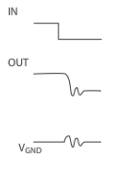
\includegraphics[width=3.00cm]{img_21.png}
\end{figure}
Diminuer le slew rate, utiliser des IC SMD ou BGA, ne pas partager les vias, diminuer l'impédance des connexions au GND
\subsection{Signaux différentiels}
Immunité aux perturbations en mode commun et aux perturbations sur le GND et moins de perturbations émises / reçues.\\
Éviter de passer des pistes proche de paires différentielles
\subsubsection{Terminaisons}
Éviter les reflections avec une terminaison égale à l'impédance de la ligne $Z_0$ (série ou parallèle).\\
\subsubsection{Parallèles}
\begin{itemize}
\item Plus de puissance
\item Moins de temps de montée/descente
\end{itemize}
\begin{figure}[H]
\centering
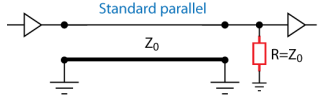
\includegraphics[width=4.00cm]{img_22.png}
\end{figure}
\subsubsection{Thévenin}
Pas recommandé pour TTL et CMOS
\begin{figure}[H]
\centering
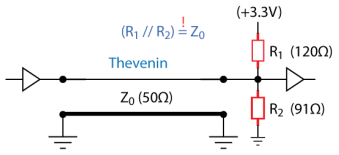
\includegraphics[width=4.00cm]{img_23.png}
\end{figure}
\subsubsection{Couplage AC}
\begin{itemize}
\item Dégrade trop les signaux d'horloge
\end{itemize}
\begin{figure}[H]
\centering
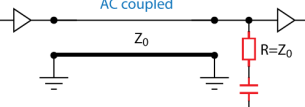
\includegraphics[width=4.00cm]{img_24.png}
\end{figure}
Terminaison côté récepteur, le niveau de commutation est fait en une seule étape, grande dissipation de puissance.
\subsubsection{Séries}
\begin{itemize}
\item Uniquement pour des connexions point-to-point
\item faible pertes
\item pour des charges avec impédance élevée
\item Grand temps de montée/descente
\end{itemize}
Pour un signal d'horloge : Buffers puis résistances séries vers la source.
\begin{figure}[H]
\centering
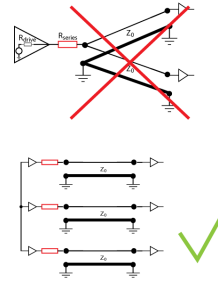
\includegraphics[width=3.00cm]{img_25.png}
\end{figure}
A utiliser pour des arbres d'horloge (avec plusieurs résistances au début)
\subsection{Routage}
Oscillateur et circuits rapides au centre du pcb, les circuits de puissance sont placés vers les alim et les régulateurs, diviser le pcb selon les composants.\\
Éviter les connexions en grilles, privilégier plus de pistes sans avoir à percer le plan de masse
\begin{figure}[H]
\centering
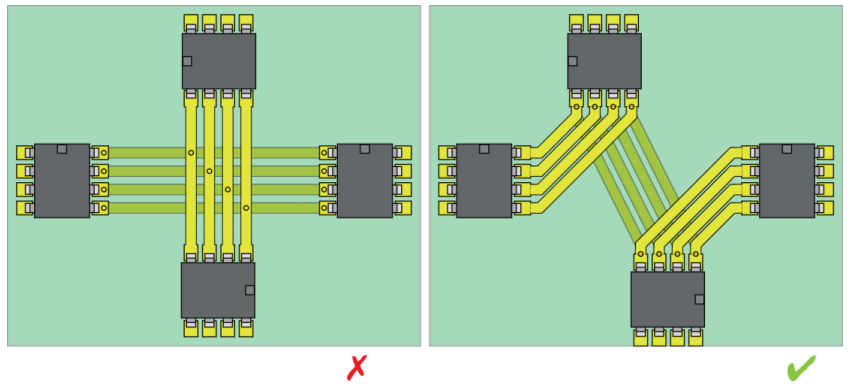
\includegraphics[width=6.00cm]{img_28.png}
\end{figure}
\subsubsection{Microvia}
diamètre $<\SI{0.15}{\milli\meter}$ et qui ne traversent pas forcément toutes les couches. Côut plus élevés mais beaucoup d'avantages. "Via-in-pad" (diminution des inductances de couplage). Moins de perforations des plans
\subsection{Choix des composants}
Pas de logique rapide (juste assez rapide pour le design), composants avec des boîtiers petits, composants avec le bon pinout(entrée d'un côté et sortie de l'autre), beaucoup de GND, vérifier la fréquence de résonance des capa de découplage

\subsection{Connectors and cables}
Câbles plats : signal aller-retour placés à côté (un GND entre chaque signal).\\
Câbles torsadés : mieux que les câbles plats sur les longues distances\\
Câbles blindés: bon contrôle de l'impédance de la ligne de transmission. Si le shield est mal câblé on perd tous les avantages\\
L'utilisation d'un choke permet de réduire les courant perturbateurs
\begin{figure}[H]
\centering
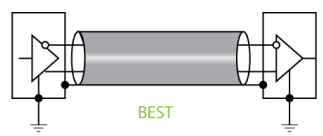
\includegraphics[width=4.00cm]{img_29.png}
\end{figure}
Impédance de transfert d'un câble :
$$Z_\text{transfer}=\frac{u_{\text{mesuré}}}{i_{\text{appliqué}}}$$
Ajouter des ferrites / chokes, connecter le blindage du câble directement au châssis
\subsection{Multi-cartes}
Toujours mieux d'avoir un système sur un seul PCB. Plusieurs cartes donnent :
\paragraph{Problèmes de lignes de transmission}
\paragraph{Crosstalk} : diminuer la distance entre les signaux et ajouter des GND entre les pistes, prévoir un GND séparé pour chaque signal et/ou diminuer l'inductance mutuelle ou la variation de courant
\paragraph{Perturbations RF} : Ajouter une plaque métallique de séparation ou prévoir une couche GND extérieure sur chaque carte. Prévoir également une manière de diminuer l'impédance GND
\paragraph{Ground bounce} : Diminuer la vitesse de transition des signaux
\paragraph{réflexions (stubs)}
\paragraph{clock skew}
\paragraph{EMI} (diminuer l'aire entre le signal et son retour)
Pour un signal très sensible et rapide, utiliser un canal LVDS (high speed serial differential channel).\\
Toujours faire un blindage au niveau PCB avant de toucher à l'armoire
\subsection{ESD}
Filtrage immédiat à l'entrée du câble dans le PCB, diminuer l'aire des boucles, bien faire attention à la mise à terre du PCB (masse chaude et froide si nécessaire).\\
Utiliser des diodes transil pour absorber les tensions.
\subsection{Testabilité}
\begin{itemize}
\item Ajouter des points de tests pour tous les nets
\item Toutes les pins de BGA doivent être accessibles depuis la face opposée
\item Prévoir des points de tests sur les alimentations de chaque IC ainsi que sur les reset
\item Prévoir de désactiver les oscillateurs
\item Connecter les entrées inutilisées au GND
\item Ajouter des résistances de \SI{0}{\ohm} pour déconnecter certaines parties
\end{itemize}
\subsection{Ferrites / Condensateurs}
\begin{itemize}
\item Condensateurs pour les signaux rapides $>\SI{10}{\mega\hertz}$ et qui varient continuellement
\item Ferrites pour les signaux à basse fréquence et/ou broadband (comme UART)
\end{itemize}
\subsection{Illustrations}
\begin{figure}[H]
\centering
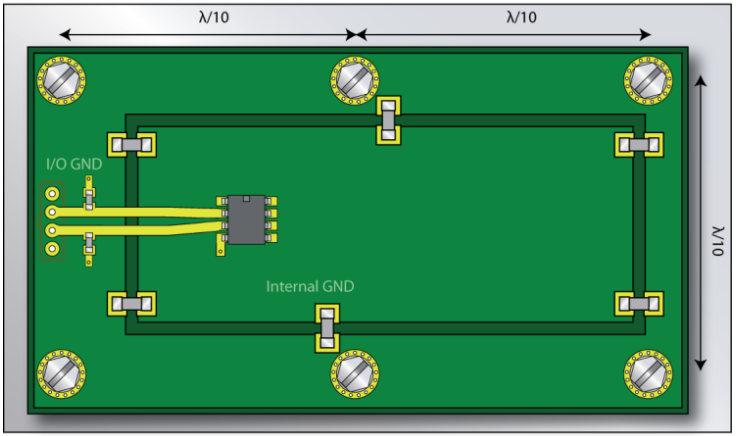
\includegraphics[width=0.9\columnwidth]{img_30.png}
\end{figure}
\begin{figure}[H]
\centering
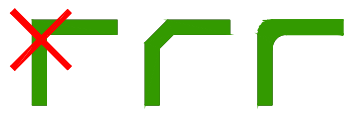
\includegraphics[width=5.00cm]{img_83.png}
\end{figure}
\subsection{Réponses aux quiz}
\begin{figure}[H]
\centering
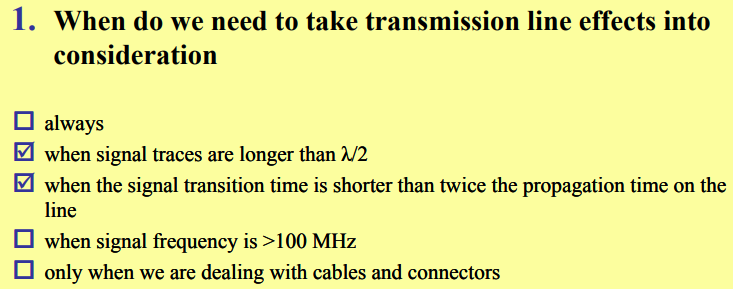
\includegraphics[width=\columnwidth]{img_84.png}
\end{figure}
\begin{figure}[H]
\centering
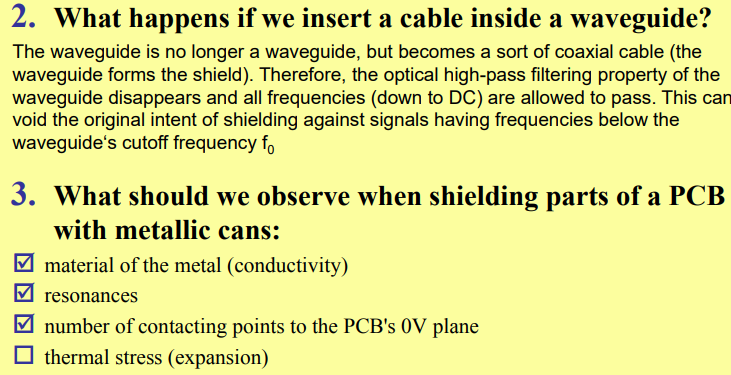
\includegraphics[width=\columnwidth]{img_85.png}
\end{figure}
\begin{figure}[H]
\centering
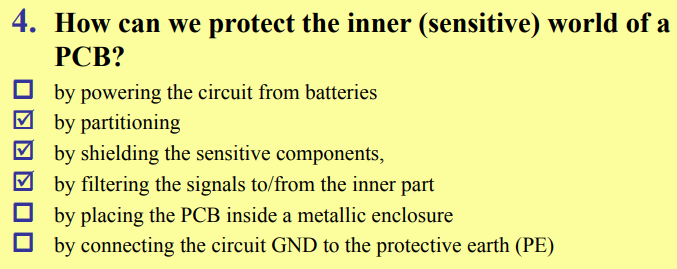
\includegraphics[width=\columnwidth]{img_86.png}
\end{figure}
\begin{figure}[H]
\centering
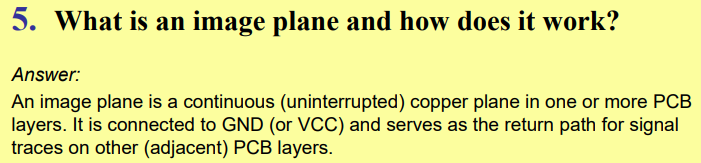
\includegraphics[width=\columnwidth]{img_87.png}
\end{figure}
\begin{figure}[H]
\centering
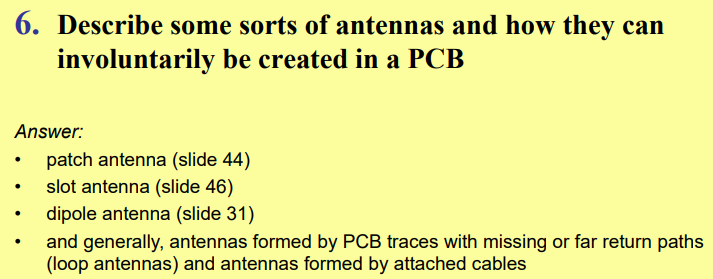
\includegraphics[width=\columnwidth]{img_88.png}
\end{figure}
\begin{figure}[H]
\centering
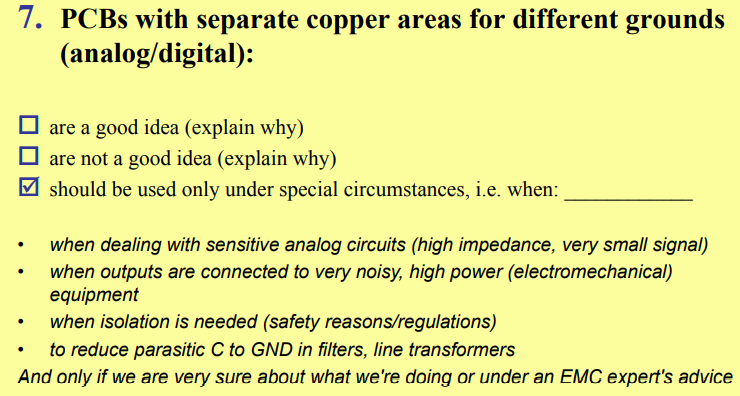
\includegraphics[width=\columnwidth]{img_89.png}
\end{figure}
\begin{figure}[H]
\centering
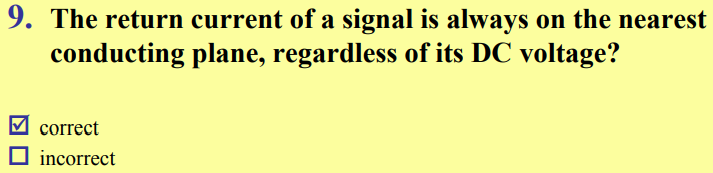
\includegraphics[width=\columnwidth]{img_90.png}
\end{figure}
\begin{figure}[H]
\centering
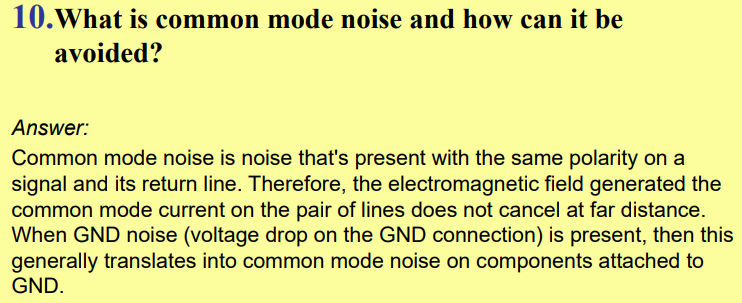
\includegraphics[width=\columnwidth]{img_91.png}
\end{figure}


\end{multicols}
\end{document}